
\documentclass[twoside]{scrarticle}
\let\tempmargin\oddsidemargin
\let\oddsidemargin\evensidemargin
\let\evensidemargin\tempmargin
\reversemarginpar

\usepackage{graphicx, float, caption}
\usepackage{amsmath} 
\begin{document}
\title{Soal Kalkulus BAB 13}
\author{Muhammad Haekal Muhyidin Al-Araby \protect\\ 5024221030}

\maketitle

\section*{Soal}
\begin{enumerate}
\item[23.] $x = t,\;y = \frac{1}{1 + t^2},\;z = t^2$

Jawab : Semua bilangan real memenuhi persamaan sehingga didapat grafik

\begin{minipage}{\linewidth}
    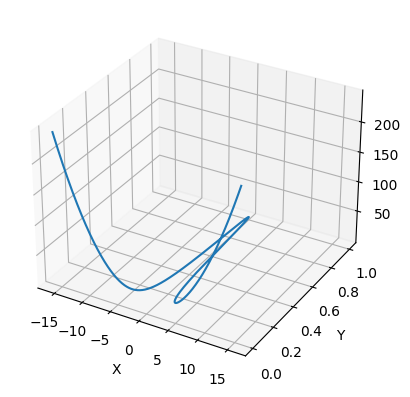
\includegraphics[width=0.5\textwidth]{image2.png}
    \centering
    \captionof{figure}{No. 23}
\end{minipage}
\item[27.] Show that the curve with parametric equations $x = t\;cos\;t,y=t\;sin\;t, z=t$ 
lies on the cone $z^2 = x^2 + y^2$, and use this fact to help sketch the curve.

Jawab: Semua bilangan real memenuhi persamaan sehingga didapat grafik, Didapat
bahwa persamaan parametrik berada pada permukaan kerucut

\begin{minipage}{\linewidth}
    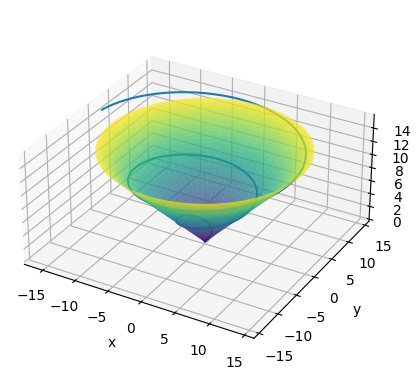
\includegraphics[width=0.5\textwidth]{27.png}
    \centering
    \captionof{figure}{No. 27}
\end{minipage}

\item[31 - 35] Use a computer to graph the curve with the given vector equation. 
Make sure you choose a parameter domain and viewpoint that reveal the true natur 
of the curve.
\item[31.] $r(t) = <cos\;t\;sin\;2t, sin\;tsin\;2t, cos\;2t>$

Jawab: Semua bilangan real memenuhi persamaan sehingga didapat grafik

\begin{minipage}{\linewidth}
    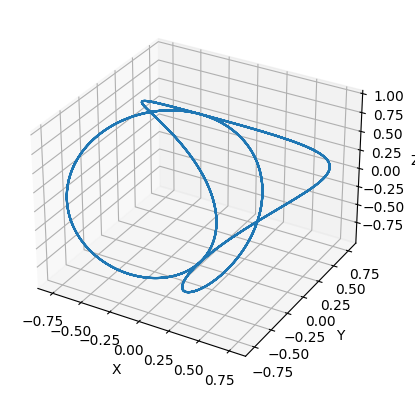
\includegraphics[width=0.5\textwidth]{31.png}
    \centering
    \captionof{figure}{No. 31}
\end{minipage}

\item[32.] $r(t) = <t^2, ln\;t, t>$

Jawab: Karena terdapat $ln\;t$ dimana t tidak boleh negatif maka domainnya adalah $t > 0$ sehingga didapat grafik

\begin{minipage}{\linewidth}
    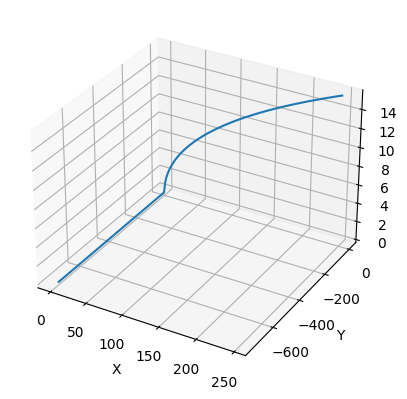
\includegraphics[width=0.5\textwidth]{32.png}
    \centering
    \captionof{figure}{No. 32}
\end{minipage}
\item[33.] $r(t) = <t, t\;sin\;t, t\;cos\;t> $

Jawab: Semua bilangan real memenuhi persamaan sehingga didapat grafik dan 
berbentuk seperti 2 kerucut horizontal yang saling berlawanan arah

\begin{minipage}{\linewidth}
    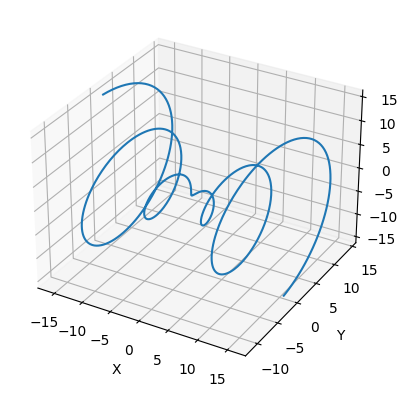
\includegraphics[width=0.5\textwidth]{33.png}
    \centering
    \captionof{figure}{No. 33}
\end{minipage}

\item[34.] $r(t) = <t, e^t, cos\;t> $

Jawab: Semua bilangan real memenuhi persamaan sehingga didapat grafik.

\begin{minipage}{\linewidth}
    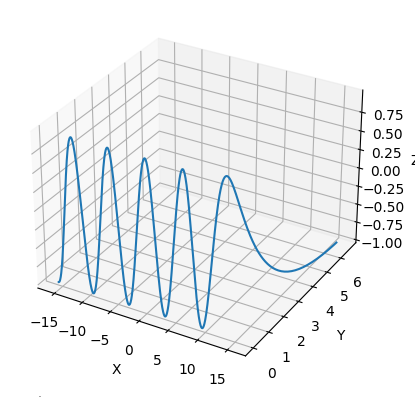
\includegraphics[width=0.5\textwidth]{34.png}
    \centering
    \captionof{figure}{No. 34}
\end{minipage}

\item[35.] $r(t) = <cos\;2t, cos\;3t, cos\;4t> $  

Jawab: Semua bilangan real memenuhi persamaan sehingga didapat grafik

\begin{minipage}{\linewidth}
    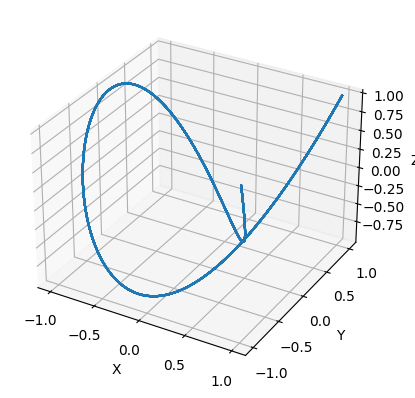
\includegraphics[width=0.5\textwidth]{35.png}
    \centering
    \captionof{figure}{No. 35}
\end{minipage}

\item[36.] Graph the curve with parametric equations $x = sin\;t, y = sin\;2t, z = cos\;3t$. 
Explain its shape by graphing its projections onto the three coordinate planes.

Jawab: Semua bilangan real memenuhi persamaan sehingga didapat grafik, 
Lalu didapat juga proyeksi pada tiga bidang koordinat untuk lebih jelas dalam
mengetahui bentuknya 

\begin{minipage}{\linewidth}
    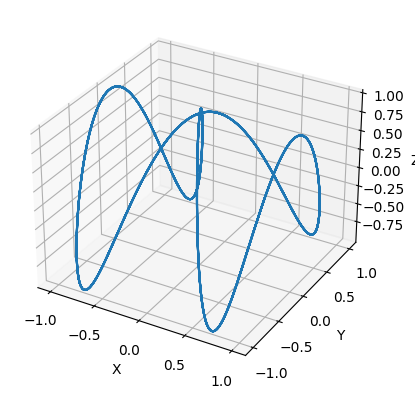
\includegraphics[width=0.5\textwidth]{36.png}
    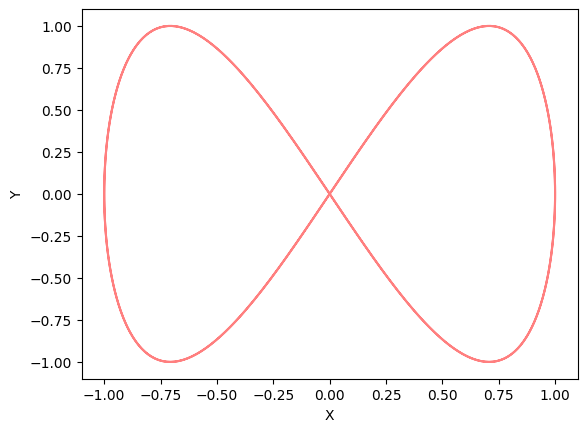
\includegraphics[width=0.5\textwidth]{36_xy.png}
    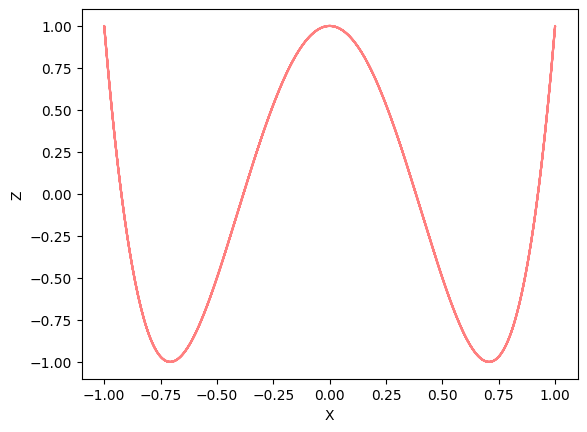
\includegraphics[width=0.5\textwidth]{36_xz.png}
    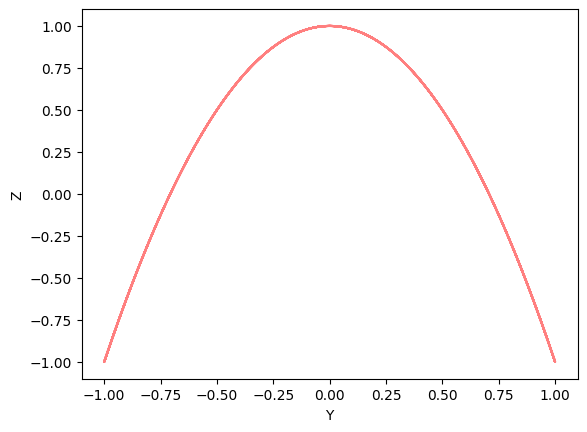
\includegraphics[width=0.5\textwidth]{36_yz.png}
    \captionof{figure}{No. 36}
\end{minipage}

\item[37.] Graph the curve with parametric equations
\begin{equation*}
    \begin{aligned}
        x & = (1+cos\;16t)\;cos\;t\\
        y & = (1+cos\;16t)\;sin\;t\\
        z & = 1 + cos\;16t
    \end{aligned}
\end{equation*}
Explain the appearance of the graph by showing that it lies on a cone

Jawab: Semua bilangan real memenuhi persamaan sehingga didapat grafik, Lalu
juga didapat bahwa persamaan parametrik tersebut terlihat seperti 
gelombang pada permukaan kerucut.

\begin{minipage}{\linewidth}
    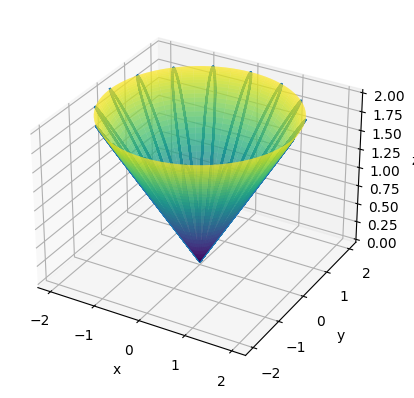
\includegraphics[width=0.5\textwidth]{37.png}
    \centering
    \captionof{figure}{No. 37}
\end{minipage}

\item[38.] Graph the curve with parametric equations
\begin{equation*}
    \begin{aligned}
        x & = \sqrt{1-0.25\;cos^2t}\;cos\;t\\
        y & = \sqrt{1-0.25\;cos^2t}\;sin\;t\\
        z & = 0.5\;cos\;10t
    \end{aligned}
\end{equation*}
Explain the appearance of the graph by showing that it lies on a sphere.

Jawab: Semua bilangan real memenuhi persamaan sehingga didapat grafik, 
Lalu didapat seperti gelombang pada permukaan bola. Bola didapat dengan plotting
Bola dengan pusat (0, 0) dan jari jari 1

\begin{minipage}{\linewidth}
    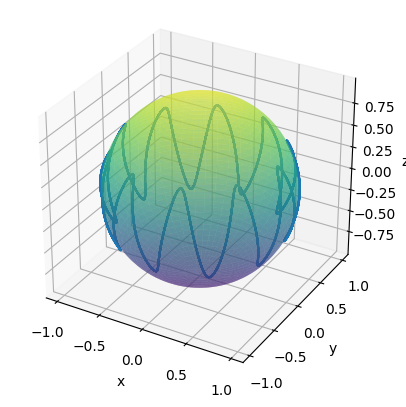
\includegraphics[width=0.5\textwidth]{38.png}
    \centering
    \captionof{figure}{No. 38}
\end{minipage}

\item[41.] The cone $z = \sqrt{x^2 + y^2}$ and the plane $z = 1+y$

Jawab: Semua bilangan real memenuhi persamaan sehingga didapat grafik, dan diketahui
bahwa bidang $z = 1 + y$ memotong kerucut $z = \sqrt{x^2 + y^2}$ 

\begin{minipage}{\linewidth}
    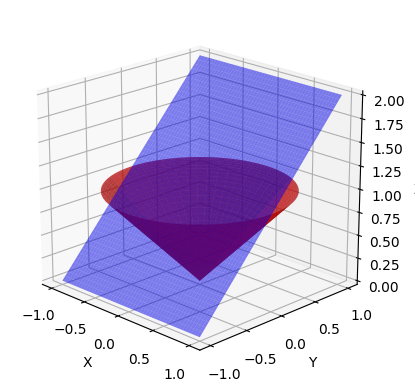
\includegraphics[width=0.5\textwidth]{41.png}
    \centering
    \captionof{figure}{No. 41}
\end{minipage}

\item[45.] Try to sketch by hand the curve of intersection of the circular cylinder 
$x^2 + y^2=4$ and the parabolic cylinder $z = x^2$. The find parametric equation for this curve and use these equations and a computer to graph the curve.

Jawab: Semua bilangan real memenuhi persamaan. Lalu didapat persamaan parametriknya
\begin{equation*}
    \begin{aligned}
        x^2 + y^2 & = 4\\
        z & = x^2\\
    \end{aligned}
\end{equation*}
\centerline{maka}
\begin{equation*}
    \begin{aligned}
        x & =2\;cos\;t\\
        y & =2\;sin\;t\\
        z & = x^2\\
          & = (2\;cos\;t)^2\\
          & = 4\;cos^2\;t\\ 
    \end{aligned}
\end{equation*}

\begin{minipage}{\linewidth}
    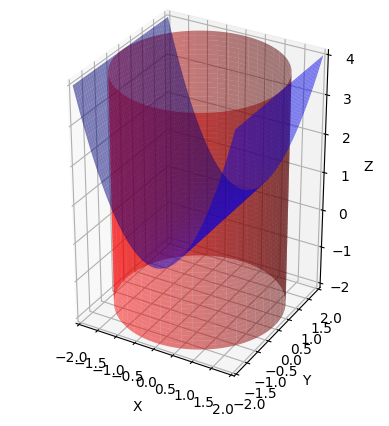
\includegraphics[width=0.5\textwidth]{45.png}
    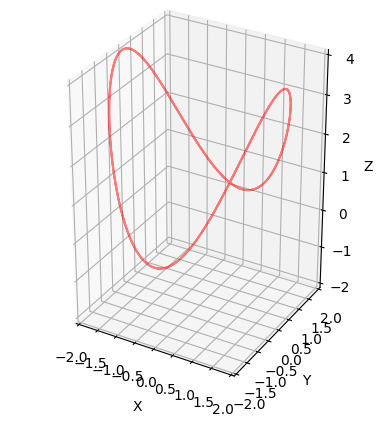
\includegraphics[width=0.5\textwidth]{45_1.png}
    \captionof{figure}{No. 45}
\end{minipage}

\item[46.] Try to sketch by hand the curve of intersection of the parabolic cylinder $y=x^2$ and the top half of the ellipsoid $x^2+4 y^2+4 z^2=16$. 
Then find parametric equations for this curve and use these equations and a computer to graph the curve.

Jawab: Semua bilangan real memenuhi persamaan. Lalu didapat persamaan parametriknya
\begin{equation*}
    \begin{aligned}
        y & = x^2\\
        x^2 + 4 y^2 + 4 z^2 & = 16\\
    \end{aligned}
\end{equation*}
\centerline{maka}
\begin{equation*}
    \begin{aligned}
        x & = t\\
        y & = t^2\\
        4z^2 & = 16 - x^2 - 4y^2\\
        z^2 & = 4 - \frac{x^2}{4} - y^2\\
        z & = \sqrt{4 - \frac{x^2}{4} - y^2}\\
        z & = \sqrt{4 - \frac{t^2}{4} - t^4}\\
    \end{aligned}
\end{equation*}

\begin{minipage}{\linewidth}
    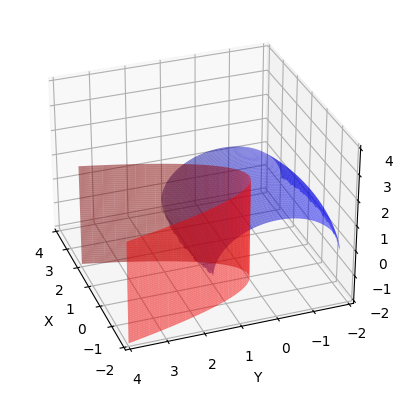
\includegraphics[width=0.5\textwidth]{46.png}
    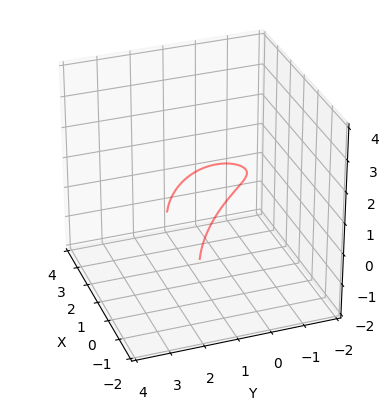
\includegraphics[width=0.5\textwidth]{46_1.png}
    \captionof{figure}{No. 46}
\end{minipage}

\item[50.] The view of the trefoil knot shown in Figure 8 is accurate, but it doesn't reveal the whole story. Use the parametric equations
$$
\begin{aligned}
& x=(2+\cos 1.5 t) \cos t \\
& y=(2+\cos 1.5 t) \sin t \\
& z=\sin 1.5 t
\end{aligned}
$$
to sketch the curve by hand as viewed from above, with gaps indicating where the curve passes over itself. Start by showing that
 the projection of the curve onto the $x y$-plane has polar coordinates $r=2+\cos 1.5 t$ and $\theta=t$, so $r$ varies between 1 and 3 . 
 Then show that $z$ has maximum and minimum values when the projection is halfway between $r=1$ and $r=3$.
When you have finished your sketch, use a computer to draw the curve with viewpoint directly above and compare 
with your sketch. Then use the computer to draw the curve from several other viewpoints. You can get a better impression of the curve 
if you plot a tube with radius 0.2 around the curve. (Use the tubeplot command in Maple or the tubecurve or Tube command in Mathematica.)

Jawab: Semua bilangan real memenuhi persamaan. Grafik dan proyeksinya terhadap ke tiga bidang adalah

\begin{minipage}{\linewidth}
    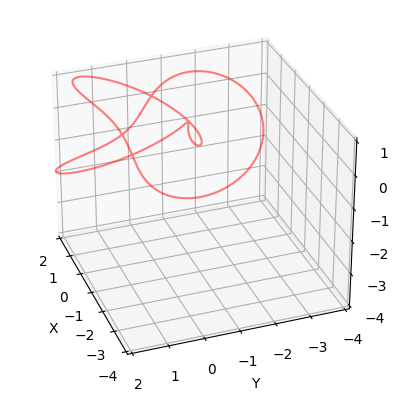
\includegraphics[width=0.5\textwidth]{50.png}
    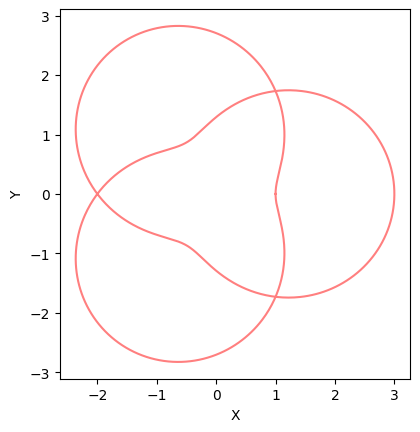
\includegraphics[width=0.5\textwidth]{50_1.png}
    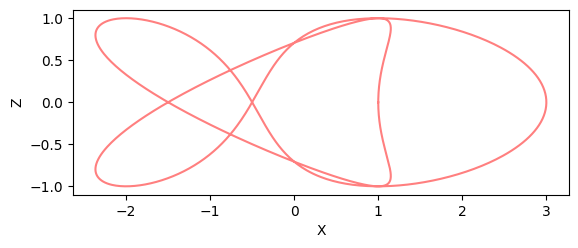
\includegraphics[width=0.5\textwidth]{50_2.png}
    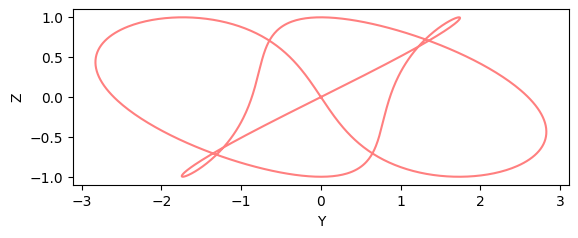
\includegraphics[width=0.5\textwidth]{50_3.png}
    \captionof{figure}{No. 50} 
\end{minipage}

didapat bahwa proyeksi pada bidang $xy$ lebih menunjukkan bentuk sebenarnya dari fungsi parametrik tersebut.

\end{enumerate}
\end{document}
